% VeriGate-FW — paper draft (P8-02). Every number cites a directory under evaluation/results/ or a
% model card; figures are the PDFs produced by evaluation/figures.py and nothing else.
% Build: latexmk -pdf main.tex   (IEEEtran; see docs/paper/README.md)
\documentclass[conference]{IEEEtran}
\usepackage[utf8]{inputenc}
\usepackage[T1]{fontenc}
\usepackage{graphicx}
\usepackage{booktabs}
\usepackage[hyphens]{url}
\urlstyle{tt}
\usepackage[hidelinks]{hyperref}
\hypersetup{pdftitle={VeriGate-FW: Verifiable AI-Gated Firmware Updates for IoT Devices with Revocable Analysis Models on a Blockchain}}
\usepackage{amsmath}
\graphicspath{{../../evaluation/figures/}}

\newcommand{\sys}{VeriGate-FW}
\newcommand{\res}[1]{{\small\path{#1}}}  % \path breaks at / and _

\begin{document}

\title{\sys: Verifiable AI-Gated Firmware Updates for IoT Devices\\ with Revocable Analysis Models on a Blockchain}

\author{\IEEEauthorblockN{Author}
\IEEEauthorblockA{Department, Institution\\ email}}

\maketitle

\begin{abstract}
Signature-based update frameworks such as Uptane establish \emph{who} produced a firmware update,
not whether a genuine update is \emph{safe} to install, and systems that add a risk analysis
treat the analyser as infallible. We present \sys{}, a software-only update gate in which a
deterministic stage (nine fail-closed checks against on-chain registries and the last approved
image) precedes an AI risk stage (an SBOM vulnerability model and a firmware-image anomaly model,
both registered on-chain by hash) whose scores an on-chain policy maps to approve, defer or
reject. Every verdict names its model hashes, commits to its features and is anchored in Merkle
batches, so a model is a revocable supply-chain artefact: revoking it marks its verdicts stale and
gateways re-verify the affected devices with the successor. Devices read publisher keys and
release records from the chain themselves, so a compromised gateway cannot install unregistered,
withdrawn or revoked-key firmware. On a laptop with a local chain, a device verification takes
128\,ms in-process, anchoring costs 1\,048 gas per verdict at 200 per batch, a revoked model's
verdicts for 50 devices are replayed in 13.0\,s, and thirteen attacks are caught in all 62 runs.
We report failures with the same care: the anomaly model misses small byte patches and section
swaps (AUROC 0.54, 0.53); a deterministic release-delta check holds all 120 such patches and
97 swaps on an unchanged base for review with no benign release flagged (0/165), but nothing
detects a patch inside a rebuild; and the learned SBOM model improves calibration, not ranking,
over a CVSS/EPSS/KEV baseline.
\end{abstract}

\begin{IEEEkeywords}
firmware update, IoT security, blockchain, IPFS, SBOM, anomaly detection, model governance
\end{IEEEkeywords}

\section{Introduction}
A vendor with tens of thousands of deployed devices cannot visit them; it ships firmware over the
air. The receiving device must decide whether the file is authentic, untampered, not an old
version replayed by an attacker, not withdrawn by the vendor, and---even when all of that holds---
not quietly shipping a library with a serious known vulnerability. The first four questions are
answered by signed metadata and a revocation record; frameworks such as The Update Framework and
Uptane~\cite{tuf,uptane} and blockchain-anchored variants~\cite{fotb,baza,didauth} do this well.
The fifth question is where those systems stop, and it is where the recent SBOM-triage
literature~\cite{sbomtriage} starts---without any binding between the analysis and the update
decision.

\sys{} closes that gap with three properties that, to our knowledge, no prior system combines:
\begin{enumerate}
\item \textbf{Two-stage gate with three outcomes.} A deterministic stage that can only reject or
defer, followed by a risk stage whose output is thresholded by an \emph{on-chain} policy into
approve, defer (human review) or reject. The AI can tighten a decision, never loosen it.
\item \textbf{Accountable verdicts.} Each verdict records the hashes of the models that produced
it and a hash of the quantised feature vector, is signed by the gateway and anchored as a Merkle
leaf on-chain, so anyone holding the model files can recompute and check it.
\item \textbf{Revocable models.} A model is registered by hash like a firmware release. Revoking
it marks every batch that used it stale; gateways swap to the registry's successor and re-verify
the affected devices automatically.
\end{enumerate}
Two deterministic mechanisms complement the AI where it is measurably weak: a
\emph{release-delta} check that holds for review an image that is the last approved image with a
few blocks overwritten or moved (the footprint of a post-build modification that no learned
detector here can see), and device-side registry checks that keep a compromised gateway from
installing anything unregistered, withdrawn or signed by a revoked key. A language model produces
a human-readable rationale for reviewers; its content is stored by content identifier in the
verdict and is never read by the decision path.

Everything is measured, and the failures are reported alongside the successes
(Section~\ref{sec:limits}). The implementation, models, fixtures, attack scripts and raw results
are released.

\section{Related work}
\label{sec:related}
TUF~\cite{tuf} and Uptane~\cite{uptane} define role-separated signed metadata with rollback and
freeze protection; they have no notion of an analysis decision and no cross-vendor audit trail.
FOTB~\cite{fotb} and Baza et al.~\cite{baza} anchor firmware fingerprints on a blockchain and
serve images from IPFS; DIDAuth-IoTFW~\cite{didauth} authenticates firmware with decentralised
identifiers and verifiable credentials on real hardware. LedgerGuard~\cite{ledgerguard} adds
SBOMs, staged roll-out and Merkle-rooted accountability of device receipts on a permissioned
ledger. The SBOM-triage pipeline of Tolay~\cite{sbomtriage} scores firmware SBOMs with CVSS,
EPSS and CISA KEV but does not connect the score to an update decision or an audit trail.
DDoSViT~\cite{ddosvit} applies a vision transformer to OTA updates, but to the \emph{network}:
it detects DDoS traffic against the update channel, not risk in the firmware being delivered,
and its model is not registered or revocable. None registers the analysis model, none can revoke it, and none combines a deterministic gate with a
three-outcome policy. The supplementary comparison table (\res{docs/comparison.md})
lists feature presence per system as described in each source.

\section{Design}
\label{sec:design}

\subsection{Actors and registries}
A \emph{publisher} holds an Ed25519 key bound to a DID in \texttt{PublisherRegistry} (register,
rotate, revoke, reputation). A release is a signed \emph{manifest}---firmware hash, SBOM hash,
semantic version, device model, expiry, IPFS CIDs, publisher DID---whose canonical JSON (a JCS
subset without floats) is signed; the release identifier is the keccak-256 of the unsigned
canonical manifest and is registered in \texttt{FirmwareRegistry}, which enforces monotonic
versions per publisher and device model, a future expiry and the publisher role. Artefacts are
content-addressed on IPFS with CIDv1 computed identically to Kubo. \texttt{ModelRegistry} holds
analysis models by SHA-256 hash with a status and an optional successor.
\texttt{PolicyContract} holds the weights and thresholds; \texttt{VerdictRegistry} holds batch
roots and answers \texttt{staleByModel}. All contracts are Solidity 0.8.26 on OpenZeppelin
\texttt{AccessControl} with custom errors and 100\,\% statement coverage.

\subsection{Stage 1: the deterministic gate}
Nine pure checks run in order and short-circuit: firmware hash, manifest signature under the
DID's registered key, publisher active, version strictly above the device's installed version,
expiry, SBOM hash, registry record not revoked, every configured model active, and the
\emph{release delta} (below). Any failure except expiry and release delta yields REJECT; an
expired manifest yields DEFER with an alert (the freeze attack). A dependency outage (chain RPC or
IPFS) yields DEFER, never APPROVE. Because the checks are pure functions of recorded inputs, a
verdict can be replayed.

\textbf{Release delta (check 9).} The reference is the newest earlier, non-revoked release of the
same publisher and device model that this gateway \emph{approved} and whose served image still
matches its on-chain hash---never a held, rejected or tampered release. Every 64-byte block of
the new image is looked up among the reference's 64-byte windows at every 4-byte offset, so code
that merely moved still matches; repeated blocks (padding, tables) must also sit where the
reference continues. If at most 32 blocks (2\,KiB) changed and the image is not byte-identical,
or blocks were reordered, the release is the approved image modified after the build and is held
for review (DEFER) with the changed offsets in the reason. A rebuild changes far more: the
smallest benign rebuild in the corpus changes 76 blocks. The check never rejects, because a vendor
binary hot-patch has the same footprint; it moves the decision to a person.

\subsection{Stage 2: the AI risk gate}
\textbf{SBOM risk.} Ten integer-quantised features (component and CVE counts, CVSS statistics,
EPSS mass, KEV count, outdatedness, dependency age) are computed from a CycloneDX SBOM with OSV,
a dated EPSS snapshot and the CISA KEV catalogue from a disk cache. A
\texttt{HistGradientBoostingRegressor} predicts the growth of the release's exposure between a
feature date $T_0$ and a label date $T_1$, where exposure is $\sum_{c} \mathrm{EPSS}_{T_1}(c)$,
the expected number of exploited CVEs; $r_\mathrm{sbom} = 1-\exp(-\hat y/6)$. The corpus is 624
real OpenWrt release manifests across 49 releases; the split is temporal (newest 20\,\% held
out)~\cite{card-sbom}.
\textbf{Image anomaly.} Fourteen pure features (chunk entropy statistics, printable ratio, ELF
header and program-header sanity, declared size, appended bytes, and deltas versus the previous
release) feed an \texttt{IsolationForest} trained on 165 benign OpenWrt ELF binaries only;
$r_\mathrm{img}$ maps the anomaly score so that the benign median is 0 and the benign 99th
percentile is 0.5. A documented, seeded mutation catalogue (byte-patch, append, section-swap,
pack, downgrade-relabel) produces the synthetic tampered set used for evaluation
only~\cite{card-img}. Both models run only as ONNX at inference; training is byte-deterministic
so the registered hashes are meaningful; SHAP attributions of the top three features are recorded
per verdict.

\subsection{Policy, reputation and verdicts}
$R = w_\mathrm{sbom} r_\mathrm{sbom} + w_\mathrm{img} r_\mathrm{img} + w_\mathrm{rep}(1-\rho)$
in basis points with weights $(0.4, 0.4, 0.2)$ and thresholds $\tau_\mathrm{approve}=0.45$,
$\tau_\mathrm{reject}=0.70$ chosen so that the three genuine fixture releases sit at approve /
defer / approve with neutral reputation~\cite{adr8}. Reputation $\rho$ is an on-chain EWMA
($\alpha=0.1$) raised by signed install receipts and lowered by release-level rejections; only
the gateway role may write it, and with $w_\mathrm{rep}=0.2$ it can move a release into DEFER but
never into REJECT by itself. The verdict record (release, device, model hashes, feature hash,
scores, $R$, verdict, rationale CID, timestamp) is signed by the gateway (EIP-191), hashed into a
domain-separated Merkle leaf and committed in batches bounded by size or time; the gateway serves
proofs and the contract verifies them. A DEFER from the policy or from check~9 can be resolved
once by a named reviewer (accept or reject, with a note); the decision is itself a signed verdict
record whose feature hash commits to the decision, the reviewer and the held verdict it resolves,
and later verdicts for the release carry it. Stage-1 rejections, expired manifests and outages
cannot be overridden.

\subsection{Model revocation}
An administrator revokes a model hash naming a successor. The gateway polls model status; on
revocation it reads \texttt{staleByModel}, joins the batch identifiers with its local batch
store (only where the Merkle root matches the chain), locates the successor \emph{by hash} under
its model directory, swaps only that scorer slot and re-runs the full gate for every stale
(release, device) pair through the normal batcher. Without a successor file the revoked hash stays
configured and Stage 1 rejects on \emph{model active}: the gate fails closed~\cite{adr9}.

\subsection{Device-side enforcement}
Before writing its inactive A/B slot, the device re-checks the firmware hash, the manifest
signature, the device model and the version. It does not take the publisher key from the gateway:
it reads the publisher record and the release record from the chain itself and requires the
publisher to be active and the release to be registered, not withdrawn, from that publisher and
for exactly this image. A compromised gateway therefore cannot make a device install code that is
unsigned, unregistered, withdrawn, downgraded or signed by a revoked key. It can still approve a
registered release the gate would have held; that verdict is anchored with its feature hash and
model hashes, so the misbehaviour is detectable afterwards rather than prevented.

\subsection{Explainer}
A local \texttt{qwen2.5:3b-instruct} via Ollama receives the SBOM diff against the previous
release, the scores and the top attributions and must answer with a schema-constrained JSON
object (summary, up to five risks, a suggested action). The validated object is pinned to IPFS
and its CID stored in the verdict. No verification waits for it: the reviewer asks for the
rationale from the console (the gateway re-runs the gate with the same models so the text
describes exactly what the gate saw), or, when configured, the gateway writes it after each
release-level verdict; the suggested action is forced to match the verdict. A missing or malformed
answer degrades to ``no rationale'', never to ``no verdict''~\cite{adr2}.

\section{Implementation}
Python 3.11 (FastAPI gateway, asyncio device emulator, Typer CLIs, structlog), Solidity/Hardhat
2.29, a React dashboard typed from the gateway's OpenAPI schema, and Docker Compose for
portability (\texttt{make up} starts the chain, IPFS, deployer, model registrar, gateway, fleet
and dashboard; \texttt{make smoke} proves a verdict from a clean machine). The fixtures are real
OpenWrt \texttt{busybox} builds (22.03.7, 23.05.3, 24.10.0 and an end-of-life 19.07.10) with
SBOMs derived from the real package manifests, so Stage-2 inputs are in the training
distribution. Thirteen attack scripts run only against the local emulated fleet. The code base has
385 unit tests (92\,\% coverage), 74 contract tests (100\,\%), 19 integration and 14 end-to-end
tests, run before every release.

\section{Evaluation}
\label{sec:eval}
All measurements are on one laptop (Intel i7-1255U, 15\,GB RAM, no GPU) against a local Hardhat
node and Kubo, with the explainer disabled unless stated; $\geq 5$ repetitions, warm-up runs
discarded, median with interquartile range; every run directory records the commit, machine,
contract addresses, model hashes and vulnerability-snapshot date. Figures are produced only by
\res{evaluation/figures.py}.

\subsection{Latency}
Fig.~\ref{fig:latency}. The nine Stage-1 checks on a fetched bundle take 3.7\,ms
(IQR 3.0--4.2); the full deterministic verification path---model status and policy reads from
the chain, the reference image, checks, record signing and batch queueing---takes 95.3\,ms warm
and 108.1\,ms when the manifest, firmware and SBOM are fetched from IPFS first
(\res{latency_stage1/2026-10-02_1702}, $n=90$ per metric). Stage 2 adds 111\,ms for SBOM scoring
and 114\,ms for image scoring the first time a release is seen and 0.1\,ms / 1.3\,ms afterwards
(per-hash caches); a complete verification for a device costs 128.2\,ms in-process (IQR
113--134) and 244\,ms over HTTP (\res{latency_stage2/2026-10-02_1702}, $n=60$). An A/B in one
session with check~9's reference lookup disabled measured 114.9\,ms and 213.5\,ms
(\res{ablation_check9_off/}), so the check costs about 10\,ms in-process and 18\,ms over HTTP;
its comparison alone takes 3.1\,ms median and at most 27\,ms over the corpus and is cached per
(release, reference) pair. The explainer is three orders of magnitude
slower: six sequential rationales took 42.5--91.3\,s each (median 88.4\,s) on the CPU
(30--33\,s with the model already loaded~\cite{adr2}), which is why no verification waits for it.

\begin{figure}[t]
\centering
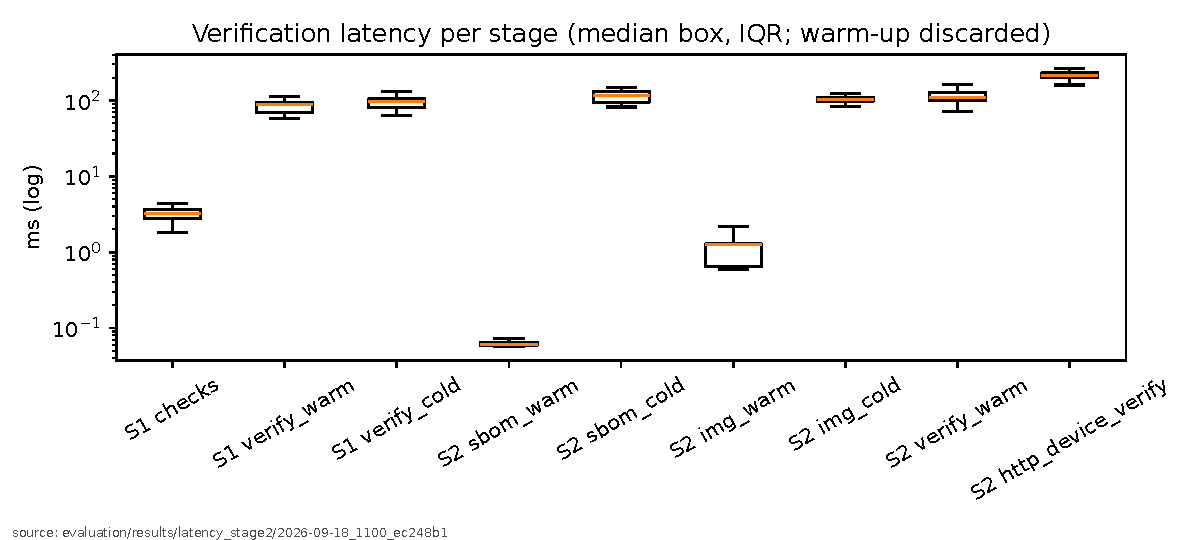
\includegraphics[width=\columnwidth]{latency.pdf}
\caption{Verification latency per stage (ms, log scale); source directories in the figure footer.}
\label{fig:latency}
\end{figure}

\subsection{Anchoring cost}
Fig.~\ref{fig:gas}. \texttt{commitBatch} costs 209\,642 gas independent of the number of
verdicts it covers (the root, the count and two model hashes are stored; leaves are not), so the
cost per verdict falls from 209\,642 with one verdict per transaction to 20\,964 at 10, 4\,193 at
50, 2\,096 at 100 and 1\,048 at 200---a 99.5\,\% reduction
(\res{gas_per_verdict_vs_batched/2026-09-18_1044}, five receipts per size). These are
\texttt{gasUsed} values from local receipts; no gas price and no L2 data-availability cost are
included. On a real rollup each transaction also pays for its calldata, which batching reduces in
the same direction but not by the same factor, so the figure above is a statement about execution
gas alone; a public-testnet measurement is left for future work.

\begin{figure}[t]
\centering
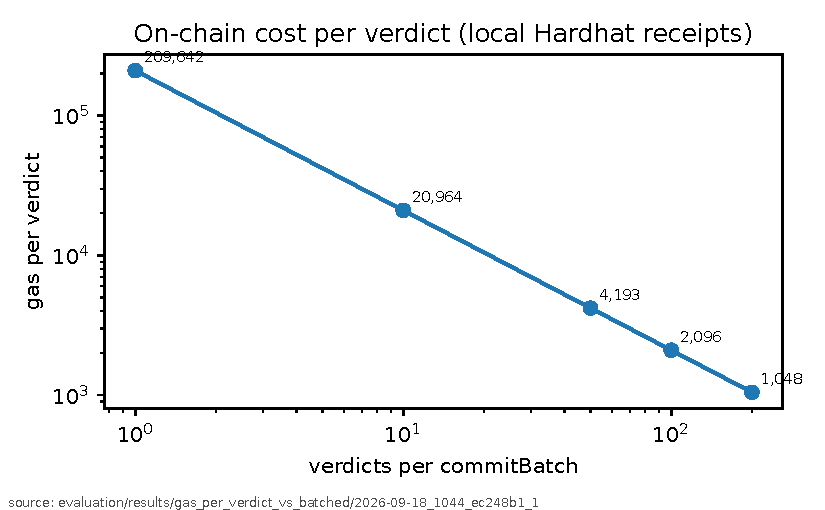
\includegraphics[width=0.85\columnwidth]{gas_per_verdict.pdf}
\caption{Gas per anchored verdict versus batch size (local Hardhat receipts).}
\label{fig:gas}
\end{figure}

\subsection{Model revocation propagation}
Fig.~\ref{fig:revocation}. After the gateway notices a revocation, replaying 5 / 20 / 50 stale
device verdicts with the successor takes 8.3 / 9.9 / 13.0\,s (IQR within 0.31\,s), to which the
2\,s poll interval adds the detection bound
(\res{revocation_propagation/2026-10-02_1704}, five repetitions per size). About 7.8\,s is the
fixed cost of loading the successor ONNX model and its SHAP background; each further device adds
roughly 100\,ms. Verdicts that used the revoked model but were not yet anchored---still queued, or
refused by \texttt{VerdictRegistry} because the model is no longer active---are taken out of the
queue and replayed too; earlier, one such verdict blocked every later batch. Every replayed verdict kept its outcome because the successor in this experiment
is the same detector retrained with another seed---the experiment measures propagation, not
detection.

\begin{figure}[t]
\centering
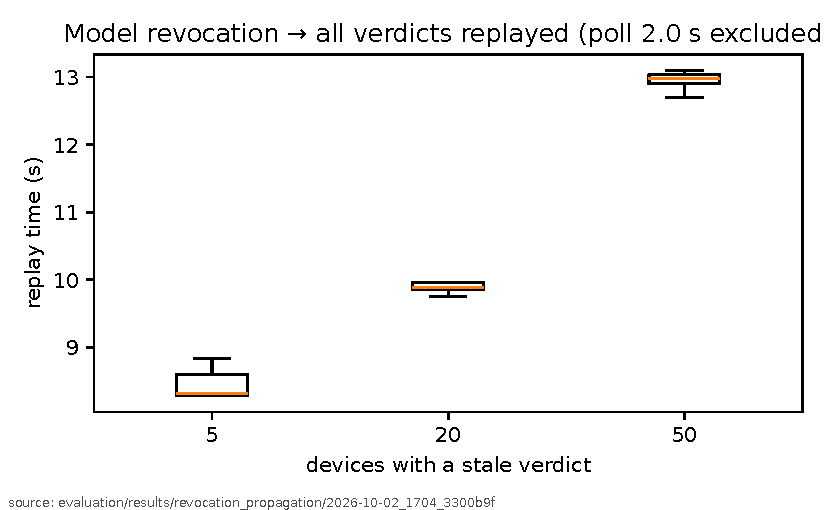
\includegraphics[width=0.85\columnwidth]{revocation_propagation.pdf}
\caption{Time from revocation detection to the last replayed verdict versus fleet size.}
\label{fig:revocation}
\end{figure}

\subsection{Attack matrix}
Table~\ref{tab:attacks}. Each scenario was run five times against the running gateway
(\res{attack_matrix/2026-10-02_1653}); \emph{poisoned-model} twice, because a model hash can
be revoked once and the shipped stack has one primary image model and one successor (the second
run revokes the successor with no replacement and every replayed verdict fails closed). In
\emph{insider patch} a fresh publisher's clean build is approved, then the same build with
256\,bytes overwritten is signed with the real key: every cryptographic check passes and check~9
holds it. In \emph{rogue gateway} a fake gateway answers a device's poll with APPROVE and pushes an
attacker-signed unregistered image, a withdrawn release and a release of a revoked publisher; the
device refuses all three from the chain records, while a genuine release pushed the same way (with
the attacker's key offered) installs. All 62 runs produced the expected outcome.

\begin{table}[t]
\caption{Attack matrix: expected outcome (observed in every run), runs and pass rate.}
\label{tab:attacks}
\centering
\footnotesize
\setlength{\tabcolsep}{4pt}
\begin{tabular}{@{}lcrr@{}}
\toprule
attack & outcome & runs & pass \\
\midrule
tamper (patched image behind the CID) & REJECT & 5 & 100\,\% \\
forge (attacker key, victim DID) & REJECT & 5 & 100\,\% \\
stolen key (revoked key) & REJECT & 5 & 100\,\% \\
rollback (older genuine release) & REJECT & 5 & 100\,\% \\
freeze (expired manifest) & DEFER & 5 & 100\,\% \\
SBOM swap (clean hash, dirty SBOM) & REJECT & 5 & 100\,\% \\
vulnerable-but-genuine (EOL base) & DEFER & 5 & 100\,\% \\
hidden payload (200\,KiB appended) & DEFER & 5 & 100\,\% \\
insider patch (256\,B, real key) & DEFER & 5 & 100\,\% \\
rogue gateway (3 pushes + control) & REFUSED & 5 & 100\,\% \\
bad history (four prior rejects) & DEFER & 5 & 100\,\% \\
policy tamper (non-admin setPolicy) & BLOCKED & 5 & 100\,\% \\
poisoned model (revoke, replay) & REPLAYED & 2 & 100\,\% \\
\bottomrule
\end{tabular}
\end{table}

\subsection{Detector quality}
\textbf{Image anomaly} (Fig.~\ref{fig:detection}, \res{detection_f1/2026-09-18_1125}, 165
benign and 165 mutated binaries per class, operating point $r_\mathrm{img}\ge0.5$): appended
payloads are detected with recall 1.000, precision 0.988 and AUROC 1.000; packing has AUROC
0.895 but recall 0.061 at the operating point; byte patches (recall / AUROC 0.012 / 0.543),
section swaps (0.015 / 0.527) and relabelled downgrades (0.000 / 0.435) are at or below chance.
The section-swap and relabel figures exclude mutations that leave the file byte-identical (29 and
120 of 165): in 120 of the 165 benign pairs OpenWrt did not rebuild the package, so the
``downgrade'' is the same file, and the original run had scored those as tampering. The benign
false-positive rate of 1.2\,\% is optimistic because the benign rows are the training rows.
Retraining the IsolationForest with check~9's delta features instead of the changed-chunk share
did not help: patch and swap recall stayed at 0.012 and 0.022 and appended-payload recall fell
from 1.000 to 0.297 (\res{delta_features_iforest/2026-10-02_1712}), which is why the release
delta is a deterministic check and not a model feature.
\textbf{Release delta} (Table~\ref{tab:delta}, \res{release_delta/2026-10-02_1619}): on the
pairs whose package was not rebuilt, check~9 holds every patched and swapped image (Wilson 95\,\%
lower bounds 0.969 and 0.962); it holds 38 of 45 relabelled downgrades, the other 7 being
byte-identical to the approved image; it flags no benign release (0/165, upper bound 0.023). On
rebuilt pairs it catches nothing, and nothing in the stack detects a 256-byte patch inside a
rebuild.
\textbf{SBOM risk} (\res{sbom_ranking/2026-09-18_1125}, 196 held-out rows from the 14 newest
releases, 200 bootstrap resamples): Spearman 0.965 for the model versus 0.976 for the
CVSS/EPSS/KEV baseline, both with AUROC 1.0 for ``$\ge 3$ expected exploited CVEs''; the model's
gain is calibration---MAE 0.167 versus 1.012 expected exploited CVEs---which is what absolute
policy thresholds need, not ranking.

\begin{table}[t]
\caption{Share of images flagged per class: check 9 (release delta), image model
($r_\mathrm{img}\ge0.5$) and either. ``Base'' = package not rebuilt; ``rebuild'' = rebuilt.}
\label{tab:delta}
\centering
\footnotesize
\setlength{\tabcolsep}{3.5pt}
\begin{tabular}{@{}llrrrr@{}}
\toprule
class & pairs & $n$ & check 9 & model & either \\
\midrule
benign & all & 165 & 0.000 & 0.012 & 0.012 \\
byte patch & base & 120 & 1.000 & 0.000 & 1.000 \\
byte patch & rebuild & 45 & 0.000 & 0.044 & 0.044 \\
section swap & base & 97 & 1.000 & 0.000 & 1.000 \\
section swap & rebuild & 39 & 0.000 & 0.051 & 0.051 \\
relabel & rebuild & 45 & 0.844 & 0.000 & 0.844 \\
append & all & 165 & 0.000 & 1.000 & 1.000 \\
pack & all & 165 & 0.000 & 0.061 & 0.061 \\
\bottomrule
\end{tabular}
\end{table}

\begin{figure}[t]
\centering
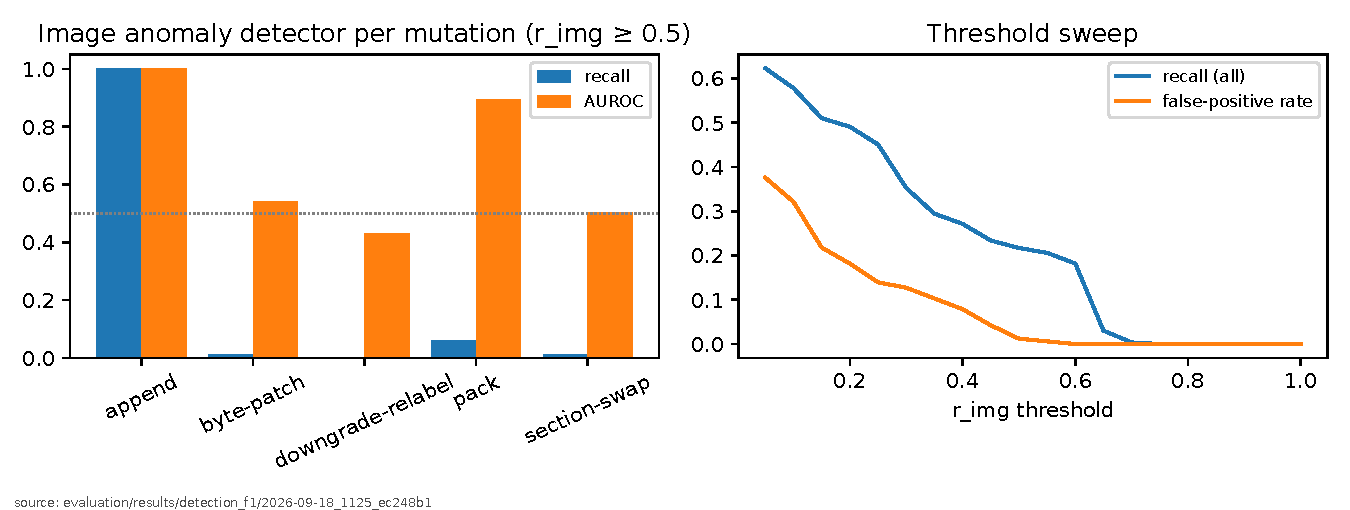
\includegraphics[width=\columnwidth]{detection_f1.pdf}
\caption{Image anomaly detector per mutation class and threshold sweep.}
\label{fig:detection}
\end{figure}

\section{Limitations}
\label{sec:limits}
Each item is backed by a measured failure (\res{docs/limitations.md}).
(i)~The image detector sees \emph{structural} tampering only; a malicious build that preserves
size, entropy and layout passes Stage 2, and detection of an appended payload depends on having
the previous release: without a predecessor the same payload scores 0.41 and the release would be
approved. Check~9 only helps when the release reuses the approved image; a modification inside a
rebuild (or a malicious source change that is then built) is invisible to every detector here,
and a genuine binary hot-patch is held for review like an attack. Its 2\,KiB limit is set from
this corpus (smallest benign rebuild 4.75\,KiB), which has no benign hot-patch releases. (ii)~No component of the OpenWrt corpus matches the CISA KEV catalogue, so the KEV
feature and the baseline's KEV floor are untested on real data; the vulnerable-but-genuine
scenario shows EPSS/CVSS mass instead. (iii)~The learned SBOM model does not out-rank the
baseline. (iv)~The explainer costs 43--91\,s per rationale on a CPU (30--33\,s warm); the full
demonstration takes 348\,s with it and 53\,s without. (v)~A model hash can be revoked once, so replay scenarios
consume models. (vi)~Release-level rejections burn the publisher's reputation and the listener's
own verification counts as a second signal, so the order of scenarios matters. (vii)~Because the
release identifier is the manifest hash, a squatter can register a predictable manifest first;
the squatted copy fails Stage 1 but the genuine publisher must re-issue with a fresh expiry.
(viii)~A compromised gateway can still approve a registered release that the gate would have
held; device-side checks prevent only unregistered, withdrawn, revoked-key and downgraded
installs, and the rest is detectable after the fact through the anchored verdict.
(ix)~Gas is local \texttt{gasUsed} only: by decision the contracts were not deployed to a public
testnet, although the deploy script targets any EVM network. The fleet is emulated rather than
run on ESP32 or Raspberry Pi hardware as in DIDAuth-IoTFW~\cite{didauth}; all timings are from
one laptop in daily use, so medians vary between runs; and the first
Stage-2 verification on an empty vulnerability cache takes about ten minutes.

\section{Conclusion}
\sys{} shows that an AI risk gate for firmware updates can be made accountable with the same
machinery that makes the firmware itself accountable: register the model by hash, name it in
every verdict, anchor the verdicts, and revoke the model when it is wrong. The deterministic
stage keeps the AI from ever loosening a decision, the on-chain policy keeps the rules auditable,
and the explain-only language model keeps the reviewer informed without touching the outcome.
Where the learned detector is measurably blind---small patches and moved sections---a
deterministic comparison with the last approved image covers the case the corpus shows to be
common, and devices that read the chain themselves keep a compromised gateway from installing
anything the registries do not vouch for. The measured costs---about 100\,ms per verification,
about a thousand gas per anchored verdict, seconds to replay a revoked model's verdicts---are
compatible with fleet-scale operation; the measured weaknesses define the work that remains,
first among them tampering inside a rebuild.

\section*{Acknowledgment}
Generative AI tools (Anthropic Claude) were used to assist with software implementation,
experiment scripting and drafting of this manuscript. The author reviewed and verified the code,
the experiments and the text, and takes full responsibility for all content and for every
reported measurement, each of which is produced by the released scripts.

\begin{thebibliography}{99}
\bibitem{tuf} J. Samuel, N. Mathewson, J. Cappos, R. Dingledine, ``Survivable key compromise in
software update systems,'' in \emph{Proc. ACM CCS}, 2010.
\bibitem{uptane} T. K. Kuppusamy, A. Brown, S. Awwad, D. McCoy, R. Bielawski, C. Mott, S. Lauzon,
A. Weimerskirch, J. Cappos, ``Uptane: Securing software updates for automobiles,'' in \emph{Proc.
ESCAR Europe}, 2016; Uptane Standard, \url{https://uptane.org}.
\bibitem{fotb} A. Yohan, N.-W. Lo, ``An over-the-blockchain firmware update framework for IoT
devices,'' in \emph{Proc. IEEE DSC}, 2018.
\bibitem{baza} M. Baza, M. Nabil, N. Lasla, K. Fidan, M. Mahmoud, M. Abdallah, ``Blockchain-based
firmware update scheme tailored for autonomous vehicles,'' in \emph{Proc. IEEE WCNC}, 2019.
\bibitem{didauth} W. M. A. B. Wijesundara, J.-S. Lee, E. Aloupogianni, D. Tith, H. Suzuki, T. Obi,
``DIDAuth-IoTFW: Decentralized firmware authentication for smart home IoT devices using
verifiable credentials,'' \emph{Internet of Things}, vol. 34, 101788, 2025.
\bibitem{ledgerguard} LedgerGuard, ``Permissioned-DLT firmware governance, artifact anchoring,
staged rollout control, and Merkle-rooted update accountability,''
\url{https://github.com/ajalkhodair-spec/ledgerguard}, 2026.
\bibitem{sbomtriage} A. Tolay, ``Automated SBOM-driven vulnerability triage for IoT firmware: A
lightweight pipeline for risk prioritization,'' arXiv:2601.01308, 2026.
\bibitem{ddosvit} M. Ali, Y. Saleem, S. Hina, G. A. Shah, ``DDoSViT: IoT DDoS attack detection
for fortifying firmware over-the-air (OTA) updates using vision transformer,'' \emph{Internet of
Things}, vol. 30, 101527, 2025.
\bibitem{card-sbom} \sys{}, model card, \path{models/sbom_risk.card.md}, 2026.
\bibitem{card-img} \sys{}, model card, \path{models/image_anomaly.card.md}, 2026.
\bibitem{adr2} \sys{} ADR-0002, ``The LLM explains; deterministic models decide,'' 2026.
\bibitem{adr8} \sys{} ADR-0008, ``Default policy parameters,'' 2026.
\bibitem{adr9} \sys{} ADR-0009, ``Model revocation: successor by hash, replay at the gateway,'' 2026.
\end{thebibliography}

\end{document}
